\section{Marco Te\'orico del prototipo}

\subsection{Online Grooming}
El online Grooming es un fen\'omeno que podr\'iamos traducir como engatusamiento y que se utiliza para describir las pr\'acticas online de ciertos adultos para ganarse la confianza de un (o una) menor fingiendo empat\'ia, cariño, etc. con fines de satisfacción sexual (como m\'inimo, y casi siempre, obtener im\'agenes del menor desnudo o realizando actos sexuales).

Por tanto est\'a muy relacionado con la pederastia y la pornograf\'ia infantil en Internet. De hecho el grooming es en muchas ocasiones la antesala de un abuso sexual \cite{grooming}.

\subsection{Caracterización del online grooming}
De acuerdo a las conversaciones analizadas por los Doctores Aditi Gupta, Ponnurangam Kumaraguru, Ashish Surekason del Instituto Tecnol\'ogico de Informaci\'on en la India reportadas en el art\'iculo  ``Characterizing pedophile conversations on the Internet using Online Grooming Web.'' \cite{articulo}, identificaron una serie de etapas y estados que las  las conversaciones pueden atravesar. Los autores marcan 6 etapas principales las cuales se describen en la tabla \ref{table:caracterizacion}.


\begin{table}[!h]

\begin{tabular}[t]{|p{15mm} |p{22mm} |p{22mm} |p{22mm} |p{20mm} |p{20mm} |p{20mm} |}
\hline
\hline
Etapas & Formaci\'on de la amistad & Formaci\'on de una relaci\'on & Evaluaci\'on de riesgos & Exclusividad & Sexual & Conclusi\'on \\
\hline
Descriptor1 & Intercambio de cuentas de correo electr\'onico, fotograf\'ias, webcam, informaci\'on & Intercambio de cuentas de correo electr\'onico, fotograf\'ias, webcam, informaci\'on & Evaluar a los padres del ni\~no, si est\'an alrededor o qui\'en puede ver su computadora & Sentir amor y expresar exclusividad & Dar descripci\'on del cuerpo y la figura & Quedar un d\'ia, una cita, hora, lugar para conocerse en persona \\
\hline
Descriptor2 &Hablar de novios/novias & Dar suaves cumplidos & Pedir al ni\~no eliminar su historial de conversaciones, asegurarse quenadie tenga la contrase\~na & Describir actividad sexual y experiencias al ni\~no &Ser novios &Discutir puntos en com\'un para una reuni\'on \\
\hline
Descriptor3 &Obtener informaci\'on del perfil y otras cuentas del ni\~no & hablar de los hobbies del a\~no, actividades e intereses & Ver si el ni\~no est\'a c\'omodo con ver a alguien mayor& Cumplidos fuertes & Intercambiar fotograf\'ias sexuales & Asegurarse de que el ni\~no ir\'a s\'olo \\
\hline
Descriptor4 & Preguntar la edad, g\'enero, localidad, nombre, informaci\'on personal, detalles familiares & Escuela, grado, tareas, n\'umero de celular & Asegurarse de que el ni\~no no es un polic\'ia & Construir confianza entre el ni\~no y el ped\'ofilo & Dar orientaci\'on sexual, cumplidos & Decidir qu\'e hacer cuando se conozcan\\
\hline
\end{tabular} \\ \\ \\
\caption{Tabla de caracterizaci\'on del comportamiento de conversaciones peligrosas}
\label{table:caracterizacion}
\end{table}

%Con base a la tabla de caracterizacion del comportamiento de las conversaciones se propuso un conjunto de frases de acuerdo a la etapa que 
%A partir de la observaci\'on de las conversaciones y de acuerdo con la descripci\'on de la matriz se listan las siguientes frases, las cuales marcan un punto de inter\'es en la identificaci\'on de los niveles 1, 2, 3, 4 y 6:





Hacemos menci\'on del nivel 5 cuya caracter\'istica es la descripci\'on sexual de las conversaciones. Este nivel ser\'a evaluado por separado en el prototipo n\'umero 2 ya que el contexto sexual da un peso mayor en la desici\'on de la API.
\textbf{•}

\section{Descripci\'on}
Prototipo que identifica y cuenta frases pertenecientes a los niveles de  formaci\'on de la amistad, formaci\'on de una relaci\'on, evaluaci\'on de riesgos, exclusividad y conclusi\'on de la caracterizac\'on del online grooming.

\section{Objetivo}
Desarrollar un prototipo que procese conversaciones de texto para buscar y contar las frases de los niveles de formaci\'on de la amistad, formaci\'on de una relaci\'on, evaluaci\'on de riesgos, exclusividad y conclusi\'on descritas en la tabla de caracterizac\'on del online grooming.


\section{An\'alisis}
\subsection{Caracter\'isticas}

\begin{description}
\item[FEAT1:] El sistema realiza la b\'usqueda de frases del nivel de formaci\'on de amistad.
\item[FEAT2:] El sistema raliza el conteo de frases del nivel de formaci\'on de amistad.
\item[FEAT3:] El sistema realiza la b\'usqueda de frases del nivel de formaci\'on de una relaci\'on.
\item[FEAT4:] El sistema raliza el conteo de frases del nivel de formaci\'on de una relaci\'on.
\item[FEAT5:] El sistema realiza la b\'usqueda de frases del nivel de evaluaci\'on de riesgos.
\item[FEAT6:] El sistema raliza el conteo de frases del nivel evaluaci\'on de riesgos.
\item[FEAT7:] El sistema realiza la b\'usqueda de frases del nivel de exclusividad.
\item[FEAT8:] El sistema raliza el conteo de frases del nivel de exclusividad.
\item[FEAT9:] El sistema realiza la b\'usqueda de frases del nivel de conclusi\'on.
\item[FEAT10:] El sistema raliza el conteo de frases del nivel conclusi\'on.
\end{description}

\subsection{Restricciones}
\begin{itemize}
\item Conversaciones alamacenadas en archivos de texto planos.
\item Conversaciones almacenadas en archivos con formato XML.
\item Implementaci\'on del prototipo en python.

\end{itemize}

\section{Dise\~no}

La figura \ref{fig:arquitectura_prototipo1} muestra la arquitectura del prototipo. Tal como se muestra en el diagrama, la entrada de informaci\'on del prototipo son los archivos que contienen a las conversaciones. La salida del prototipo ser\'an los valores del n\'umero de frases correspondientes a cada nivel de caracterizaci\'on del Online grooming. Estos valores ser\'an almacenados en una base da datos para su posterioir procesamiento y análisis.



	\begin{figure}[!h]
	\begin{center}
	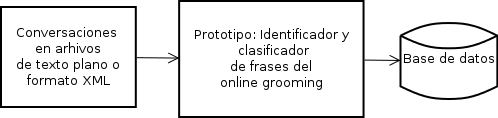
\includegraphics[scale=.5]{images/arquitectura_prototipo1}
	\caption{Arquitectura del prototipo 1}
	\label{fig:arquitectura_prototipo1}
	\end{center}
	\end{figure}


\subsection{Diagrama de Clases}


La figura \ref{fig:diagramaDeClase} muestra el diagrama de la clase que conforma el prototipo. Los atributos de cada clase representan el n\'umero de frases que la conversaci\'on tiene en el nivel que describe.
\begin{figure}[h]
	\begin{center}
	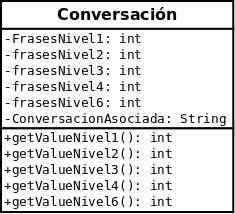
\includegraphics[scale=.4]{images/claseprotipo2}
	\caption{Diagrama de Clase del prototipo 1}
	\label{fig:diagramaDeClase}
	\end{center}
	\end{figure}



\subsection{M\'etodo para la identificaci\'on y conteo de frases del nivel de formaci\'on de amistad}
La siguiente lista de frases pertenecen al nivel de formaci\'on de amistadad cuyo objetivo es establecer confianza y obtener datos de la v\'ictima. Estas frases se seleccionaron de acuerdo a las posibles frases que se pod\'ian formar de acuerdo a los descriptores que la tabla de caracterizac\'on muestra.

\begin{itemize}
\item ?`C\'omo te llamas?
\item ?`C\'ual es tu nombre?
\item ?`Cu\'antos a\~nos tienes?
\item ?`D\'onde vives?
\item ?`Qu\'e m\'usica te gusta?
\end{itemize}


El siguiente c\'odigo muestra mediante la cual detectamos las frases que corresponden al nivel 1. Para hacer la b\'usqueda se toman palabras clave como palabras anclas y as\'i poder encontrar no s\'olo la frase escrita integramente sino que tambi\'en se puedan identificar algunos de sus derivados.

\begin{lstlisting}[language=Python]
def detectarNivel1(self):	
		for mensaje in self.mensajes:
			#Contexto busqueda de la edad
			if (u'cuantos' in mensaje) == True:
				if(u'anos' in mensaje) == True:
					if(u'tienes' in mensaje) == True:
				#		print mensaje
						self.nivel1 += 1
	
			if(u'cual' in mensaje) == True:
				if(u'edad' in mensaje) == True:
				#	print mensaje
					self.nivel1 += 1
			#Contexto busqueda nombre
			if(u'como' in mensaje) == True:
				if(u'llamas' in mensaje) == True:
				#	print mensaje
					self.nivel1 += 1
			if(u'cual' in mensaje) == True:
				if(u'nombre' in mensaje)== True:
				#	print mensaje
					self.nivel1 += 1
			if(u'donde' in mensaje) ==  True:
				if(u'vives' in mensaje) == True:
				#	print mensaje
					self.nivel1 += 1
			if(u'musica' in mensaje) == True:
					self.nivel1 += 1
			if(u'escuchar' in mensaje) == True:
					self.nivel1 += 
\end{lstlisting}



\subsection{Lista de frases de nivel formaci\'on de una relaci\'on}
La siguiente lista de frases son frases que pertenecen al nivel de formaci\'on de una relaci\'on de la tabla de caracterizaci\'on del online grooming, cuyo objetivo es establecer amistad con la v\'ictima. 
Las frases fueron propuestas de acuerdo a los descriptores que el nivel marca.

\begin{itemize}
\item ?`Tienes Fotos?
\item ?`Tienes webcam?
\item ?`En qu\'e escuela vas?
\item ?`Cu\'al es tu celular?
\item ?`Cu\'al es tu tel\'efono?
\item ?`Cu\'al es tu n\'umero telef\'onico?
\end{itemize}

\begin{lstlisting}[language=Python]
def detectarNivel2(self):
		stemmer = SnowballStemmer("spanish")
		for mensaje in self.mensajes:
			for palabra in mensaje:
				#Contecto fotos
				if stemmer.stem(palabra) == stemmer.stem("tienes"):
					for palabra2 in mensaje:
						if stemmer.stem(palabra2) == stemmer.stem("fotos"):
				#			print mensaje
							self.nivel2 += 1
				
					for palabra2 in mensaje:
						if stemmer.stem(palabra2) == stemmer.stem("camara"):
				#			print mensaje
							self.nivel2 += 1
					
					for palabra2 in mensaje:
						if stemmer.stem(palabra2) == stemmer.stem("webcam"):
				#			print mensaje
							self.nivel2 += 1
					
					for palabra2 in mensaje:
						if stemmer.stem(palabra2) == stemmer.stem("celular"):
						#	print mensaje	
							self.nivel2 += 1
				#Contexto Escuela
				elif stemmer.stem(palabra) == stemmer.stem("escuela"):
				#	print mensaje
					self.nivel2 +=1		
				elif stemmer.stem(palabra) == stemmer.stem("cual"):	
					for palabra2 in mensaje:
						if stemmer.stem(palabra2) == stemmer.stem("numero"):
						#	print mensaje	
							self.nivel2 += 1
						if stemmer.stem(palabra2) == stemmer.stem("telefono"):
						#	print mensaje	
							self.nivel2 += 1	
						if stemmer.stem(palabra2) == stemmer.stem("celular"):
						#	print mensaje	
							self.nivel2 += 1


\end{lstlisting}

\subsection{Lista de frases de nivel evaluaci\'on de riesgos}
La siguiente lista de frases son frases que pertenecen al nivel 3 de caracterizaci\'on, cuyo objetivo es conocer la situaci\'on y relacion de la v\'ictima con sus padres o familiares.  


\begin{itemize}
\item ?`D\'onde est\'a tu mam\'a?
\item ?`D\'onde est\'a tu pap\'a?
\item ?`Tus pap\'as trabajan?
\end{itemize}

\begin{lstlisting}[language=Python]
def detectarNivel3(self):
		stemmer = SnowballStemmer("spanish")
		for mensaje in self.mensajes:
			for palabra in mensaje:
				#Padres
				if (stemmer.stem(palabra) == stemmer.stem("padres")) or (stemmer.stem(palabra) == stemmer.stem("papa")) or (stemmer.stem(palabra) == stemmer.stem("mama")) or (stemmer.stem(palabra) == stemmer.stem("padres")) or (stemmer.stem(palabra) == stemmer.stem("madre")): 
					for palabra2 in mensaje:
						if(palabra2 == "tu") or (palabra2 == "mis") or (palabra2 == "mi") or (palabra2 ==  "tus") or (palabra2 =="tu"):
							self.nivel3 += 1
							if self.nivel3 >= 3:
								self.nivel3_2 +=1 
	
\end{lstlisting}

\subsection{Lista de frases de nivel exclusividad}
La siguiente lista de frases son frases que pertenecen al nivel 4 de caracterizaci\'on, cuyo objetivo es establecer vinculos de novizago o alg\'un tipo de relaci\'on. 


\begin{itemize}
\item ?`Quieres ser mi novia?
\item ?`Quieres ser mi novio?
\item Eres bonita o bonito.
\item Eres guapo.
\item Me gustas. 
\item Eres hermosa.
\end{itemize}

\begin{lstlisting}[language=Python]
def detectarNivel4(self):
		stemmer = SnowballStemmer("spanish")
		for mensaje in self.mensajes:
			for palabra in mensaje:
				if palabra == "eres":
					for palabra2 in mensaje:
						if (stemmer.stem(palabra2) == stemmer.stem("bonita")) or (stemmer.stem(palabra2) == stemmer.stem("sexy")) or (stemmer.stem(palabra2) == stemmer.stem("hermoso")):
#							print mensaje
							self.nivel4 += 1
				if stemmer.stem(palabra) == stemmer.stem("novio"):
					for palabra2 in mensaje:
						if palabra2 == "ser":
							print mensaje	
							self.nivel4 += 1

\end{lstlisting}
\subsection{Lista de frases de nivel conclusi\'on}
La siguiente lista de frases pertenecen al nivel 6. Este nivel tiene como objetivo establecer contacto con la v\'ictima, haciendo citas o alg\'un tipo de reuni\'on. Al igual que los niveles anteriores las frases seleccionadas aqu\'i fueron elegidas de acuerdo a un analisis basado en la observaci\'on de las conversaciones traducidas.


\begin{itemize}
\item Quiero verte
\item ?`D\'onde nos vemos?
\item Te veo en este lugar.
\item Hay que reunirnos.
\end{itemize}

\begin{lstlisting}[language=Python]
def detectarNivel6(self):
		stemmer = SnowballStemmer("spanish")
		for mensaje in self.mensajes:
			for palabra in mensaje:
				if (stemmer.stem("podemos") == stemmer.stem(palabra)) or (stemmer.stem(palabra) ==stemmer.stem("quiero")) or (stemmer.stem(palabra) == stemmer.stem("tenemos")):
					for palabra2 in mensaje:
						if (stemmer.stem(palabra2) == stemmer.stem("vernos")) or (stemmer.stem(palabra2) == stemmer.stem("verte")) or (stemmer.stem(palabra2) == stemmer.stem("reunirnos")) or (palabra2 == "ver"):
							self.nivel6 += 1
			for palabra in mensaje:
				if(palabra == "donde"):
					for palabra2 in mensaje:
						if (stemmer.stem(palabra2) == stemmer.stem("vemos")) or (stemmer.stem(palabra2) == stemmer.stem("verte")) or (stemmer.stem(palabra2) == stemmer.stem("reunirnos")) or (palabra2 == "ver"):
							self.nivel6 += 1
\end{lstlisting}
							
	
\section{Pruebas}

Se realiz\'o el an\'alis de 50 conversaciones que marcamos como peligrosas extraidas del portal \url{http://www.perverted-justice.com/}, el cual es un sitio donde se hacen p\'ublicas conversaciones que han servido de anzuelo para capturar ped\'ofilos en internet. Estas conversaciones fueron traducidas al espa\~nol y se anexan en el ap\'endice \ref{app:conversaciones}. De igual forma se marcaron 50 conversaciones no peligrosas extraidas de pl\'aticas personales de facebook anexadas en el ap\'endice \ref{app:conversacionesnp}. La tabla \ref{table:resultadosNiveles} muestra los resultados obtenidos despu\'es de an\'alisar ambos conjuntos de conversaciones.



\begin{center}
\begin{longtable}{|l|l|l|l|l|l|}

\hline
Conversaci\'on & Nivel 1 & Nivel 2 & Nivel 3 & Nivel 4 & Nivel 6 \\
\hline
\endfirsthead

\hline
Conversaci\'on & Nivel 1 & Nivel 2 & Nivel 3 & Nivel 4 & Nivel 6 \\
\hline
\endhead

\multicolumn{5}{c}{Sigue en la página siguiente.}
\endfoot

\endlastfoot

conversaciones\_txt/8.txt & 2 & 3 & 1 & 0 & 0 \\
\hline
conversaciones\_txt/29.txt & 0 & 0 & 2 & 3 & 2 \\
\hline
conversaciones\_txt/31.txt & 0 & 0 & 1 & 3 & 0 \\
\hline
conversaciones\_txt/6.txt & 1 & 2 & 3 & 2 & 0 \\
\hline
conversaciones\_txt/25.txt & 4 & 4 & 5 & 0 & 0 \\
\hline
conversaciones\_txt/cp4.txt & 0 & 1 & 2 & 0 & 1 \\
\hline
conversaciones\_txt/cp2.txt & 2 & 7 & 10 & 3 & 1 \\
\hline
conversaciones\_txt/15.txt & 0 & 0 & 0 & 0 & 1 \\
\hline
conversaciones\_txt/38.txt & 1 & 0 & 8 & 1 & 1 \\
\hline
conversaciones\_txt/40.txt & 0 & 0 & 1 & 0 & 1 \\
\hline
conversaciones\_txt/34.txt & 0 & 3 & 0 & 1 & 0 \\
\hline
conversaciones\_txt/7.txt & 0 & 2 & 1 & 2 & 0 \\
\hline
conversaciones\_txt/20.txt & 1 & 0 & 0 & 0 & 2 \\
\hline
conversaciones\_txt/cp6.txt & 0 & 1 & 5 & 3 & 3 \\
\hline
conversaciones\_txt/9.txt & 0 & 1 & 3 & 0 & 0 \\
\hline
conversaciones\_txt/13.txt & 0 & 0 & 2 & 0 & 1 \\
\hline
conversaciones\_txt/4.txt & 1 & 1 & 1 & 1 & 1 \\
\hline
conversaciones\_txt/cp3.txt & 2 & 3 & 14 & 0 & 2 \\
\hline
conversaciones\_txt/23.txt & 1 & 1 & 1 & 0 & 0 \\
\hline
conversaciones\_txt/cp1.txt & 0 & 3 & 7 & 1 & 0 \\
\hline
conversaciones\_txt/36.txt & 0 & 2 & 8 & 1 & 0 \\
\hline
conversaciones\_txt/3.txt & 0 & 1 & 0 & 0 & 0 \\
\hline
conversaciones\_txt/cp7.txt & 0 & 7 & 5 & 1 & 2 \\
\hline
conversaciones\_txt/22.txt & 0 & 0 & 1 & 0 & 0 \\
\hline
conversaciones\_txt/26.txt & 0 & 0 & 0 & 1 & 0 \\
\hline
conversaciones\_txt/32.txt & 0 & 0 & 0 & 0 & 0 \\
\hline
conversaciones\_txt/21.txt & 0 & 0 & 0 & 2 & 0 \\
\hline
conversaciones\_txt/11.txt & 0 & 1 & 2 & 0 & 0 \\
\hline
conversaciones\_txt/30.txt & 1 & 2 & 4 & 0 & 0 \\
\hline
conversaciones\_txt/39.txt & 0 & 1 & 1 & 0 & 0 \\
\hline
conversaciones\_txt/1tx.txt & 2 & 4 & 0 & 1 & 3 \\
\hline
conversaciones\_txt/18.txt & 1 & 1 & 6 & 0 & 1 \\
\hline
conversaciones\_txt/28.txt & 0 & 0 & 3 & 0 & 0 \\
\hline
conversaciones\_txt/14.txt & 0 & 1 & 0 & 0 & 1 \\
\hline
conversaciones\_txt/12.txt & 0 & 0 & 0 & 0 & 1 \\
\hline
conversaciones\_txt/5.txt & 0 & 0 & 0 & 0 & 0 \\
\hline
conversaciones\_txt/2.txt & 0 & 1 & 2 & 0 & 2 \\
\hline
conversaciones\_txt/10.txt & 0 & 1 & 5 & 0 & 0 \\
\hline
conversaciones\_txt/33.txt & 0 & 0 & 0 & 3 & 1 \\
\hline
conversaciones\_txt/17.txt & 0 & 0 & 0 & 0 & 0 \\
\hline
conversaciones\_txt/19.txt & 0 & 3 & 3 & 0 & 3 \\
\hline
conversaciones\_txt/24.txt & 1 & 0 & 0 & 1 & 0 \\
\hline
conversaciones\_txt/16.txt & 0 & 3 & 4 & 0 & 0 \\
\hline
conversaciones\_txt/27.txt & 0 & 0 & 0 & 0 & 0 \\
\hline
conversaciones\_txt/35.txt & 0 & 0 & 6 & 2 & 0 \\
\hline
conversaciones\_txt/37.txt & 0 & 0 & 0 & 0 & 1 \\
\hline
np/cnp21.txt & 0 & 0 & 0 & 0 & 0 \\
\hline
np/cnp14.txt & 0 & 2 & 0 & 0 & 0 \\
\hline
np/cnp17.txt & 1 & 1 & 0 & 1 & 0 \\
\hline
np/cnp13.txt & 0 & 0 & 0 & 0 & 0 \\
\hline
np/cnp11.txt & 0 & 2 & 0 & 0 & 0 \\
\hline
np/cnp3.txt & 0 & 1 & 0 & 0 & 0 \\
\hline
np/cnp10.txt & 0 & 2 & 0 & 0 & 0 \\
\hline
np/cnp9.txt & 1 & 1 & 0 & 0 & 0 \\
\hline
np/cnp6.txt & 0 & 0 & 2 & 0 & 0 \\
\hline
np/cnp22.txt & 0 & 2 & 0 & 0 & 0 \\
\hline
np/cnp16.txt & 0 & 3 & 0 & 0 & 1 \\
\hline
np/cnp4.txt & 0 & 1 & 0 & 1 & 0 \\
\hline
np/cnp15.txt & 0 & 7 & 4 & 0 & 1 \\
\hline
np/cnp8.txt & 0 & 1 & 0 & 0 & 0 \\
\hline
np/cnp5.txt & 0 & 1 & 0 & 0 & 0 \\
\hline
np/cnp1.txt & 0 & 4 & 1 & 0 & 3 \\
\hline
np/cnp20.txt & 0 & 0 & 0 & 0 & 0 \\
\hline
np/cnp19.txt & 0 & 3 & 0 & 0 & 0 \\
\hline
np/cnp18.txt & 0 & 2 & 0 & 0 & 0 \\
\hline
np/cnp2.txt & 0 & 1 & 2 & 0 & 1 \\
\hline
np/cnp12.txt & 0 & 2 & 0 & 0 & 1 \\
\hline
\pagebreak
np/cnp7.txt & 0 & 1 & 1 & 0 & 0 \\ 
\hline

\caption{Resultados de incidencias de Niveles 1, 2, 3, 4 y 6 }
\label{table:resultadosNiveles}
\end{longtable}
\end{center}




La gr\'afica \ref{fig:graficanopeligrosa} muestra la estad\'istica de valores de frecuencia obtenidos de la suma de todas las frecuencias de las conversaciones que hemos etiquedo como "peligrosas".

\begin{figure}[h]
\begin{center}
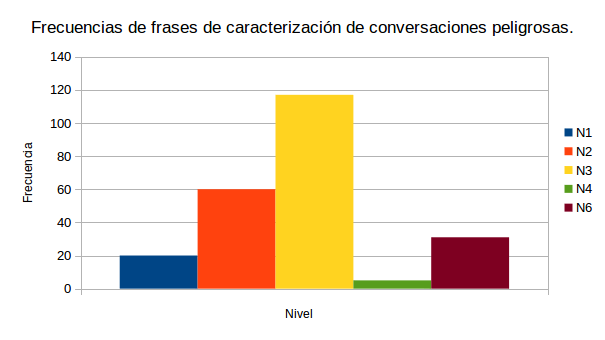
\includegraphics[scale=1]{images/graficanivelespeligrosas}
\caption{Gr\'afica de frecuencias de niveles de conversaciones peligrosas}
\label{fig:graficapeligrosa}
\end{center}
\end{figure}

La gr\'afica \ref{fig:graficanopeligrosa} muestra la estad\'istica de valores de frecuencia obtenidos de la suma de todas las frecuencias de las conversaciones que hemos etiquedo como conversaciones no peligrosas. 

\begin{figure}[h]
\begin{center}
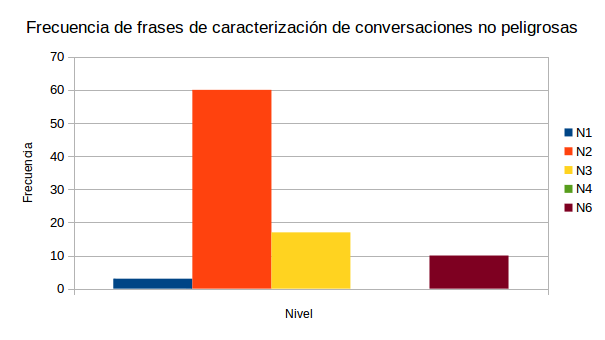
\includegraphics[scale=1]{images/graficanivelesnopeligrosas}
\caption{Gr\'afica de frecuencias de niveles de conversaciones peligrosas}
\label{fig:graficanopeligrosa}
\end{center}
\end{figure}

Haciendo la comparaci\'on de ambas gr\'aficas, se puede observar que  hay presencia de frases de nivel formaci\'on de amistad en ambos tipos de conversaciones, teniendo mayor la frecuencia de este nivel las conversaciones peligrosas.  

En el caso de la formaci\'on de relaci\'on se present\'o un comportamiento donde las conversaciones que marcamos como no peligrosas tienen casi la misma frecuencia que las conversaciones marcadas como peligrosas. Para el caso de frases de nivel de evaluaci\'on de riesgo, donde el objetivo es conocer informaci\'on de los padres, la frecuencia de frases de este nivel es mayor en las de tipo peligrosas, ya que se tiene una frecuencia de 117 a 14 de las no peligrosas. 

El nivel de conclusi\'on se present\'o con una mayor frecuencia en conversaciones peligrosas, esta diferencia es de m\'as del doble comparando un tipo de conversaci\'on con el otro.

Tanto el nivel de reconocimiento del riesgo como de conlusi\'on son niveles donde la diferencia de frecuencias es muy marcada. Pudiendo ser estos niveles aquellos que marcan la diferencia entre un tipo de conversaci\'on y otro. 
